%
% Bphi1.tex -- degree 1 spline wavelet
%
% (c) 2019 Prof Dr Andreas Müller, Hochschule Rapperswil
%
\documentclass[tikz]{standalone}
\usepackage{amsmath}
\usepackage{times}
\usepackage{txfonts}
\usepackage{pgfplots}
\usepackage{csvsimple}
\usetikzlibrary{arrows,intersections,math}
\begin{document}
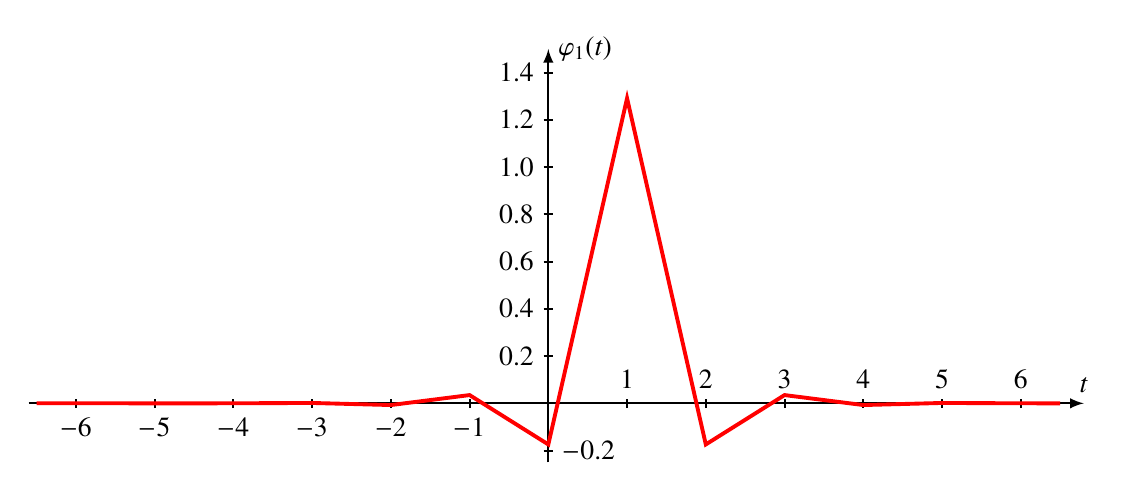
\begin{tikzpicture}[>=latex,yscale=3]

\draw[->,line width=0.7pt] (-6.6,0)--(6.8,0)
	coordinate[label={$t$}];
\draw[->,line width=0.7pt] (0,-0.25)--(0,1.5)
	coordinate[label={right:$\varphi_1(t)$}];

\foreach \t in {1,...,6}{
	\draw[line width=0.7pt] ({-\t},-0.02)--({-\t},0.02);
	\node at ({-\t},-0.02) [below] {$-\t$};
	\draw[line width=0.7pt] ({\t},-0.02)--({\t},0.02);
	\node at ({\t},0.02) [above] {$\t$};
}

\begin{scope}
\clip (-6.5,-0.2) rectangle (6.5,1.5);
\draw[line width=1.4pt,color=red]
	(-12,0.000564)
	--(-11,-0.000282)
	--(-10,0.000564)
	--(- 9,-0.000281)
	--(- 8,0.000562)
	--( -7,-0.000275)
	--( -6,0.000537)
	--( -5,-0.000172)
	--( -4,0.000118)
	--( -3,0.001566)
	--( -2,-0.007311)
	--( -1,0.034928)
	--(  0,-0.174099)
	--(  1,1.291394)
	--(  2,-0.174099)
	--(  3,0.034928)
	--(  4,-0.007311)
	--(  5,0.001566)
	--(  6,0.000118)
	--(  7,-0.000172)
	--(  8,0.000537)
	--(  9,-0.000275)
	--( 10,0.000562)
	--( 11,-0.000281)
	--( 12,0.000564)
	--( 13,-0.000282)
	--( 14,0.000564)
	--( 15,-0.000282);
\end{scope}

\draw[line width=0.7pt] (-0.06,-0.2)--(0.06,-0.2);
\draw[line width=0.7pt] (-0.06,0.2)--(0.06,0.2);
\draw[line width=0.7pt] (-0.06,0.4)--(0.06,0.4);
\draw[line width=0.7pt] (-0.06,0.6)--(0.06,0.6);
\draw[line width=0.7pt] (-0.06,0.8)--(0.06,0.8);
\draw[line width=0.7pt] (-0.06,1.0)--(0.06,1.0);
\draw[line width=0.7pt] (-0.06,1.2)--(0.06,1.2);
\draw[line width=0.7pt] (-0.06,1.4)--(0.06,1.4);

\node at ( 0.06,-0.2) [right] {$-0.2$};
\node at (-0.06,0.2) [left] {$0.2$};
\node at (-0.06,0.4) [left] {$0.4$};
\node at (-0.06,0.6) [left] {$0.6$};
\node at (-0.06,0.8) [left] {$0.8$};
\node at (-0.06,1.0) [left] {$1.0$};
\node at (-0.06,1.2) [left] {$1.2$};
\node at (-0.06,1.4) [left] {$1.4$};

\end{tikzpicture}
\end{document}

